\documentclass[tikz,border={0.2cm 0.2cm}]{standalone}
\usepackage{siunitx}
\usetikzlibrary{calc}
\begin{document}
    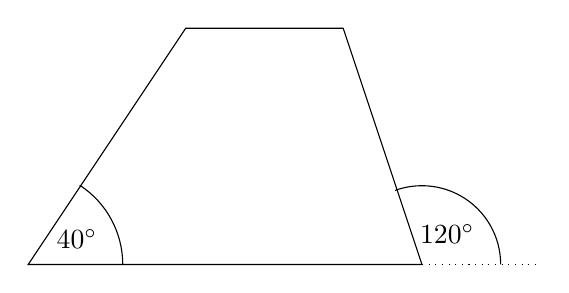
\begin{tikzpicture}
        % Meghatározzuk a trapéz csúcsainak koordinátáit
        \coordinate (A) at (0,0) {};
        \coordinate (B) at (5,0) {};
        \coordinate (C) at (4,3) {};
        \coordinate (D) at (2,3) {};
        % Megrajzoljuk a trapéz oldalait
        \draw (A) -- (B) -- (C) -- (D) -- cycle;
        % Megrajzoljuk az A csúcsnál lévő szög ívét
        \draw ($(A)+(0:1.2cm)$) arc (0:57:1.2cm);
        % Beleírjuk a szög értékét
        \node at ($(A)+(28:0.7cm)$) {$\ang{40}$};
        % Meghosszabbítjuk az AB oldalt B-n túl pontozott vonallal
        \draw[dotted] (B) -- ++(1.5,0);
        % Megrajzoljuk a B csúcsnál lévő külső szöget
        \draw ($(B)+(0:1cm)$) arc (0:110:1cm);
        % Beírjuk a szög értékét
        \node at ($(B)+(50:0.5cm)$) {$\ang{120}$};
    \end{tikzpicture}
\end{document}
